\chapter{Feasibility}

\section{Technic Feasibility}
The computer on which the project is to be developed should be at a level that meets the minimum system requirements for application development. Accordingly, the minimum system requirements for a computer to be used for application development are as follows :

\begin{itemize}
    \item JDK 1.8
    \item Spring Tool Suit, Spring Boot
    \item Eclipse, Android Studio etc. Java IDE
    \item Sublime text, gedit etc. text editor
    \item A Browser to render HTML and Javascript
    \item Android Emulator 
    \item 8 GB RAM minimum, 16 GB RAM recommended
	\item Intel Core i5 4th generation + or more powerful CPU
	\item Minimum 250GB Free Disk Space    
    \item Linux, Windows or Mac Operating System.
    
\end{itemize}


\section{Labor Force Feasibility}
Two people are currently developing the application, this is the minimum number.



\section{Time Feasibility}
\begin{figure}[!htbp]
\centering
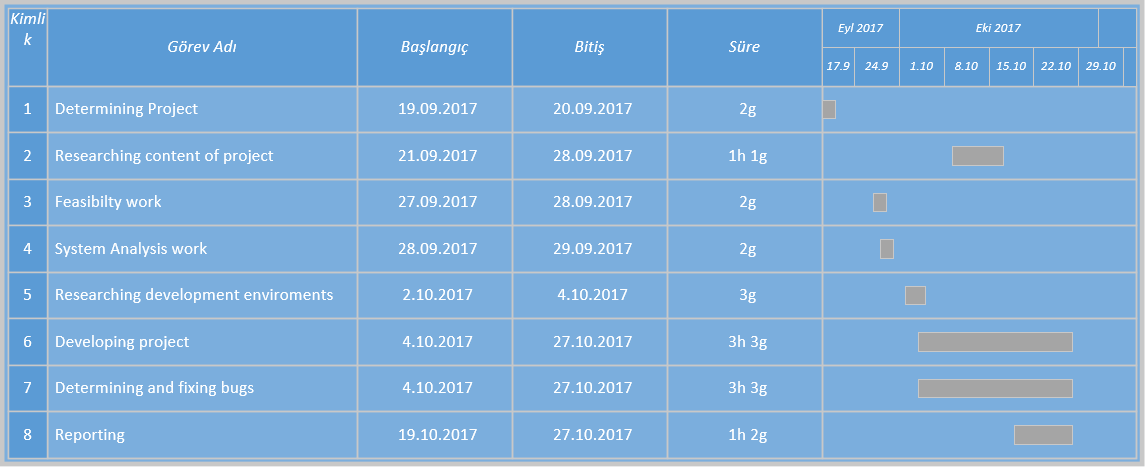
\includegraphics[width=\textwidth]{projectChapters/images/gantt.png}
\caption{Gantt Diyagramı Zaman Çizelgesi}
\end{figure}


\section{Legitimate Feasibility}
There are no patent infringements as the software components to be used in the development phase of the project are open source and free of charge. Users are responsible for the legal problems that may arise due to the shares they have made according to Article 8 of Law No. 5651 and Article 125 of the Turkish Penal Code.


\section{Economic Feasibility}
There is no charge for software components to be used during application development. The hourly working fee of the person who will develop the project is 25 TL per person. The total cost determined for the project during the project development period stated in the Gantt Chart is 8000 TL. The price of a computer with minimum system requirements stated in the title of hardware feasibility which costs currently between 1500 and 2500 TL.




